%%%%%%%%%%%%%%%%%%%%%%%%%%%%%%%%%%%%%%%%%%%%%%%%%%%%%%%%%%%%%%%%%%%%%%%%%%%%%%%%
%%%%%%%%%%%%%%%%%%%%%%%%%%%%%%%%%%%%%%%%%%%%%%%%%%%%%%%%%%%%%%%%%%%%%%%%%%%%%%%%
%%%%%%%%%%%%%%%%%%%%%%%%%%%%%%%%%%%%%%%%%%%%%%%%%%%%%%%%%%%%%%%%%%%%%%%%%%%%%%%%
%%%%%%%%%%%%%%%%%%%%%%%%%%%%%%%%%%%%%%%%%%%%%%%%%%%%%%%%%%%%%%%%%%%%%%%%%%%%%%%%
\chapter[Représentation d'état]
{Initiation à la représentation d'état\label{chap-repreEtat}}
%%%%%%%%%%%%%%%%%%%%%%%%%%%%%%%%%%%%%%%%%%%%%%%%%%%%%%%%%%%%%%%%%%%%%%%%%%%%%%%%
%%%%%%%%%%%%%%%%%%%%%%%%%%%%%%%%%%%%%%%%%%%%%%%%%%%%%%%%%%%%%%%%%%%%%%%%%%%%%%%%
%%%%%%%%%%%%%%%%%%%%%%%%%%%%%%%%%%%%%%%%%%%%%%%%%%%%%%%%%%%%%%%%%%%%%%%%%%%%%%%%
%%%%%%%%%%%%%%%%%%%%%%%%%%%%%%%%%%%%%%%%%%%%%%%%%%%%%%%%%%%%%%%%%%%%%%%%%%%%%%%%
\minitoc
\newpage
%%%%%%%%%%%%%%%%%%%%%%%%%%%%%%%%%%%%%%%%%%%%%%%%%%%%%%%%%%%%%%%%%%%%%%%%%%%%%%%%
%%%%%%%%%%%%%%%%%%%%%%%%%%%%%%%%%%%%%%%%%%%%%%%%%%%%%%%%%%%%%%%%%%%%%%%%%%%%%%%%
%%%%%%%%%%%%%%%%%%%%%%%%%%%%%%%%%%%%%%%%%%%%%%%%%%%%%%%%%%%%%%%%%%%%%%%%%%%%%%%%
\section{Contexte}
%%%%%%%%%%%%%%%%%%%%%%%%%%%%%%%%%%%%%%%%%%%%%%%%%%%%%%%%%%%%%%%%%%%%%%%%%%%%%%%%
%%%%%%%%%%%%%%%%%%%%%%%%%%%%%%%%%%%%%%%%%%%%%%%%%%%%%%%%%%%%%%%%%%%%%%%%%%%%%%%%
%%%%%%%%%%%%%%%%%%%%%%%%%%%%%%%%%%%%%%%%%%%%%%%%%%%%%%%%%%%%%%%%%%%%%%%%%%%%%%%%
Dans les précédents chapitres, les systèmes linéaires dynamiques ont été 
largement étudiés à l'aide de la notion de fonction de transfert. Cette fonction
de transfert est une représentation dans le domaine de Laplace du système que
l'on souhaite analyser, modéliser et controler. Elle permet de donner
une réprésentation fréquentielle de l'équation différentielle régissant le 
système. L'analyse des propriétés de cette fonction de transfert est riche de
résultats et nous a permis de caractériser un grand nombre des performances
des~\glspl{slci} ainsi que les performances liées à leur asservissement. 
Cependant, cette approche s'avère difficile à mettre en oeuvre dans le cas 
des systèmes non-linéaires et/ou discrets. Le but de ce chapitre est 
d'introduire une nouvelle approche  pour l'étude des systèmes dynamiques 
permettant d'englober un plus grand nombre de situation. 

Il faut également remarquer que nous avons étudié uniquement les systèmes
monovariables, il est possible de s'attaquer à l'étude des systèmes 
multivariables par l'approche fréquentielle, mais les problèmes deviennent
très rapidement difficile à étudier pour un nombre d'entrée et de sortie.   
%%%%%%%%%%%%%%%%%%%%%%%%%%%%%%%%%%%%%%%%%%%%%%%%%%%%%%%%%%%%%%%%%%%%%%%%%%%%%%%%
%%%%%%%%%%%%%%%%%%%%%%%%%%%%%%%%%%%%%%%%%%%%%%%%%%%%%%%%%%%%%%%%%%%%%%%%%%%%%%%%
\subsection{Système multivariable}
%%%%%%%%%%%%%%%%%%%%%%%%%%%%%%%%%%%%%%%%%%%%%%%%%%%%%%%%%%%%%%%%%%%%%%%%%%%%%%%%
%%%%%%%%%%%%%%%%%%%%%%%%%%%%%%%%%%%%%%%%%%%%%%%%%%%%%%%%%%%%%%%%%%%%%%%%%%%%%%%%
Au contraire des systèmes monovariables, les systèmes multivariables présentent
plusieurs entrées et sorties (en nombre différents dans le cas général)
\footnote{Il ne faut pas confondre un système
multivariable avec les systèmes multientrées que nous avons rencontré lorsque
par exemple nous avons considéré la prise en compte d'une perturbation dans
un système composé de plusieurs sous-systèmes.}. Nous pouvons représenté ce 
type de système par le schéma suivant :
%-------------------------------------------------------------------------------
\begin{center}
    \tikzsetnextfilename{mimo-ext}
    \begin{tikzpicture}
    \sbEntree{E}
    \node [above of=E, node distance=2em,coordinate, name=E1] {};
    \node [below of=E, node distance=2em,coordinate, name=E2] {};
    \node [draw, rectangle,
           minimum height=6em, minimum width=6em, right of = Edroite,
           node distance=4em,sbStyleBloc,right] (B) {\Huge$\Sigma$};
    \node (Bdroite) at (B.east){};
    \node (BlocdeFindroite) at (B.east){};
    \node [right of=E1, node distance=4em,coordinate, name=EB1] {};
    \node [right of=E2, node distance=4em,coordinate, name=EB2] {};
    \sbRelier[$e_1(t)$]{E1}{EB1}
    \sbRelier[$\vdots$]{E}{B}
    \sbRelier[$e_n(t)$]{E2}{EB2}
    \sbSortie[4]{S}{B}
    \node [above of=S, node distance=2em,coordinate, name=S1] {};
    \node [below of=S, node distance=2em,coordinate, name=S2] {};
    \node [right of=E1, node distance=10em,coordinate, name=SB1] {};
    \node [right of=E2, node distance=10em,coordinate, name=SB2] {};
    \sbRelier[$s_1(t)$]{SB1}{S1}
    \sbRelier[$\vdots$]{B}{S}
    \sbRelier[$s_n(t)$]{SB2}{S2}
\end{tikzpicture}

\end{center}
%-------------------------------------------------------------------------------
Pour un tel système de $n$ entrées/sorties, 
toutes les équations différentielles sont couplées. 
C'est à dire que l'équation différentielle d'une sortie $s_i(t)$ quelconque 
dépend de toutes les entrées $e_j(t)\quad\forall j\in[0,n]$. En passant 
directement dans le domaine de 
Laplace, on peut écrire un système d'équations reliant les sorties $S_i(p)$ 
à toutes les entrées $E_j(p)$, tel que  :
%-------------------------------------------------------------------------------
\begin{align*}
    S_1(p) =& H_{11}(p) E_1(p) + \ldots + H_{1n}(p) E_n(p) \\
    \vdots =& \\ 
    S_n(p) =& H_{n1}(p) E_1(p) + \ldots + H_{nn}(p) E_n(p)
\end{align*}
%-------------------------------------------------------------------------------
où $H_{ij}$ sont les fonctions de transfert couplant l'entrée $j$ à la sortie 
$i$. Il est alors possible de considérer le système comme une matrice 
de fonctions de transfert :
%-------------------------------------------------------------------------------
\begin{align*}
    \begin{pmatrix} 
        S_1(p)\\
        \vdots\\
        S_n(p)
    \end{pmatrix}=
    \begin{pmatrix} 
        H_{11}(p) & H_{12}(p) &\ldots & H_{1n}(p) \\
        H_{21}(p) & H_{22}(p) &\ldots & H_{2n}(p) \\
        \vdots    & \vdots    &\ldots & \vdots    \\ 
        H_{n1}(p) & H_{n2}(p) &\ldots & H_{nn}(p) 
    \end{pmatrix}\cdot
    \begin{pmatrix} 
        E_1(p)\\
        \vdots\\
        E_n(p)
    \end{pmatrix}
\end{align*}
%-------------------------------------------------------------------------------
Prenons le cas de 2 équations différentielles couplées $n=2$, on obtient 
le système d'équations  :
%-------------------------------------------------------------------------------
\begin{align*}
    S_1(p) &= H_{11}(p) E_1(p) + H_{12}(p) E_2(p) \\
    S_2(p) &= H_{11}(p) E_1(p) + H_{22}(p) E_2(p)
\end{align*}
%-------------------------------------------------------------------------------
ou dans sa forme matricielle, 
%-------------------------------------------------------------------------------
\begin{align*}
    \begin{pmatrix} 
        S_1(p)\\
        S_2(p)
    \end{pmatrix}=
    \begin{pmatrix} 
        H_{11}(p) & H_{12}(p) \\
        H_{21}(p) & H_{22}(p) 
    \end{pmatrix}\cdot
    \begin{pmatrix} 
        E_1(p)\\
        E_2(p)
    \end{pmatrix}
\end{align*}
%-------------------------------------------------------------------------------
%%%%%%%%%%%%%%%%%%%%%%%%%%%%%%%%%%%%%%%%%%%%%%%%%%%%%%%%%%%%%%%%%%%%%%%%%%%%%%%%
%%%%%%%%%%%%%%%%%%%%%%%%%%%%%%%%%%%%%%%%%%%%%%%%%%%%%%%%%%%%%%%%%%%%%%%%%%%%%%%%
\subsubsection*{Exemple}
%%%%%%%%%%%%%%%%%%%%%%%%%%%%%%%%%%%%%%%%%%%%%%%%%%%%%%%%%%%%%%%%%%%%%%%%%%%%%%%%
%%%%%%%%%%%%%%%%%%%%%%%%%%%%%%%%%%%%%%%%%%%%%%%%%%%%%%%%%%%%%%%%%%%%%%%%%%%%%%%%
Prenons l'exemple de deux équations différentielles couplées :
\[
\begin{cases}
\hphantom{\devi{s_2(t)}{2}+3}\devi{s_1(t)}{}+ s_1(t)  &=  e_1(t) + 3e_2(t) \\
          \devi{s_2(t)}{2}+3 \devi{s_2(t)}{}+ 2s_2(t) &= 2e_1(t) +  e_2(t)
\end{cases}
\]
Nous avons ici deux équations différentielles (une 1er et une du 2nd ordre).
Le système matriciel devient :
\[
    \begin{pmatrix} 
        S_1(p)\\
        S_2(p)
    \end{pmatrix}=
    \begin{pmatrix} 
    \dfrac{1}{p+1}      & \dfrac{3}{p+1} \\[2em] 
    \dfrac{2}{p^2+3p+2} & \dfrac{1}{p^2+3p+2} 
    \end{pmatrix}\cdot
    \begin{pmatrix} 
        E_1(p)\\
        E_2(p)
    \end{pmatrix}
\]
en associant les fonctions de transfert de la matrice au fonctions de transferts
de couplage $H_{ij}$, il est possible de représenter le système par le graphe 
de fluence suivant :
%-------------------------------------------------------------------------------
%\begin{align*}
%    H_{11}(p) &= \dfrac{1}{p+1}\\
%    H_{12}(p) &= \dfrac{3}{p+1}\\
%    H_{21}(p) &= \dfrac{2}{p^2+3p+2} \\
%    H_{22}(p) &= \dfrac{1}{p^2+3p+2}, 
%\end{align*}
%-------------------------------------------------------------------------------
%il est possible de représenter le système par le graphe de fluence suivant :
%-------------------------------------------------------------------------------
\begin{center}
    \tikzsetnextfilename{gf-mimo-ext}
    \begin{tikzpicture}
    \gfEntree[0][0][]{}{E}
    \gfEntree[0][3][+]{$E_1$}{E1}
    \gfEntree[0][-3][-]{$E_2$}{E2}
    \gfSortie[4]{$S_1$}[+]{E1}{S1}
    \gfSortie[4]{}[]{E}{S}
    \gfSortie[4]{$S_2$}[-]{E2}{S2}
    \gfRelier[$H_{11}$][+][1.2]{E1}{S1}
    \gfRelier[$H_{21}$][+][1.2]{E1}{S2}
    \gfRelier[$H_{12}$][-][1.2]{E2}{S1}
    \gfRelier[$H_{22}$][-][1.2]{E2}{S2}
\end{tikzpicture}

\end{center}
%-------------------------------------------------------------------------------
\clearpage
%%%%%%%%%%%%%%%%%%%%%%%%%%%%%%%%%%%%%%%%%%%%%%%%%%%%%%%%%%%%%%%%%%%%%%%%%%%%%%%%
%%%%%%%%%%%%%%%%%%%%%%%%%%%%%%%%%%%%%%%%%%%%%%%%%%%%%%%%%%%%%%%%%%%%%%%%%%%%%%%%
%%%%%%%%%%%%%%%%%%%%%%%%%%%%%%%%%%%%%%%%%%%%%%%%%%%%%%%%%%%%%%%%%%%%%%%%%%%%%%%%
\section{\'Etat d'un système dynamique}
%%%%%%%%%%%%%%%%%%%%%%%%%%%%%%%%%%%%%%%%%%%%%%%%%%%%%%%%%%%%%%%%%%%%%%%%%%%%%%%%
%%%%%%%%%%%%%%%%%%%%%%%%%%%%%%%%%%%%%%%%%%%%%%%%%%%%%%%%%%%%%%%%%%%%%%%%%%%%%%%%
%%%%%%%%%%%%%%%%%%%%%%%%%%%%%%%%%%%%%%%%%%%%%%%%%%%%%%%%%%%%%%%%%%%%%%%%%%%%%%%%
\newcommand{\bdx}{\boldsymbol{x}}
\newcommand{\bds}{\boldsymbol{s}}
\newcommand{\bde}{\boldsymbol{e}}
\newcommand{\bdt}{\boldsymbol{(t)}}
\newcommand{\bdxt}{\bdx\bdt}
\newcommand{\bdst}{\bds\bdt}
\newcommand{\bdet}{\bde\bdt}
L'étude d'un système dynamique basée sur une approche fréquentielle (c.-à-d. 
dans le domaine de Laplace) est pratique dans le cas des systèmes continus, 
linéaires et monovariables. \textbf{La représentation d'état} des systèmes 
dynamiques, que nous allons maintenant présenter, conserve une description 
naturellement temporelle de ces systèmes et pourra d'ailleurs s'appliquer 
à des systèmes dynamiques plus généraux que les seuls~\gls{slci}. 
Nous allons cependant, nous limiter à une présentation
liminaire de cette notion qui pourrait faire l'objet d'un ouvrage dédié

La représentation d'état nécessite la description d'un état 
$\bdxt$ à instant $t$\footnote{Nous utilisons ici la notation anglosaxonne qui
représente les vecteurs par des symboles en caractères gras.} qui est un 
vecteur de variables $x_i(t)$ dont le nombre $n$ de composantes dépend 
de l'ordre du système.
%-------------------------------------------------------------------------------
\begin{align*}
    \bdxt = \begin{pmatrix}
            x_1(t)\\
            \vdots\\
             x_n(t)
            \end{pmatrix}
\end{align*}
%-------------------------------------------------------------------------------
Il faut noter que le choix des variables $x_i(t)$ n'est pas unique, seul leur
nombre $n$ est fixé par le système. Ce choix correspond en toute rigueur
à choisir une base de représentation de l'état d'un système. Il est tout à 
fait possible de passer d'une représentation à une autre par une transformation
linéaire analogue à un changement de base.


Connaissant cet état $\boldsymbol{A}$ à un instant $t$, ainsi que l'entrée 
$\bdet$, il est possible de déterminer l'état du système à un 
instant $t+\dd{t}$ $\bdx\boldsymbol{(t+\dd{t})}$. \textbf{L'équation d'état} 
qui donne l'évolution de l'état du système est de la forme générale :
%-------------------------------------------------------------------------------
\begin{bequation}[ams align]
    \boldsymbol{\dot{x}}\bdt= \boldsymbol{A}\bdxt + \boldsymbol{B} \bdet
    \label{eq-etat}
\end{bequation}
%-------------------------------------------------------------------------------
où $\boldsymbol{A}$ et $\boldsymbol{B}$ sont des matrices dans le cas
général.
Dans le cas où le système est monovariable et donc que $s(t)$ et $e(t)$ sont
de simples fonctions, $\boldsymbol{A}$ est une matrice que l'on nomme la 
\textbf{matrice d'évolution}, et $\boldsymbol{B}$ est le 
\textbf{vecteur commande}.

La sortie d'un système dynamique $\bdst$ est un vecteur (dans le cas général) 
qui dépend à la fois du vecteur d'entrée $\bdet$ et du vecteur d'état $\bdxt$. 
La relation entre ces vecteurs est donnée par \textbf{l'équation de sortie} ou
\textbf{équation de mesure}:
%-------------------------------------------------------------------------------
\begin{bequation}[ams align]
    \bdst=\boldsymbol{C} \bdxt + \boldsymbol{D} \bdet
    \label{eq-sortie}
\end{bequation}
%-------------------------------------------------------------------------------
où $\boldsymbol{C}$ et $\boldsymbol{D}$ sont des matrices dans le cas
général.
Dans le cas où le système est monovariable et donc que $s(t)$ et $e(t)$ sont
de simples fonctions, $\boldsymbol{C}$ est un vecteur l'on nomme le 
\textbf{vecteur observation}, et $\boldsymbol{D}$ un simple scalaire 
\textbf{d'action directe ou de transmission} de l'entrée sur la sortie.
%%%%%%%%%%%%%%%%%%%%%%%%%%%%%%%%%%%%%%%%%%%%%%%%%%%%%%%%%%%%%%%%%%%%%%%%%%%%%%%%
%%%%%%%%%%%%%%%%%%%%%%%%%%%%%%%%%%%%%%%%%%%%%%%%%%%%%%%%%%%%%%%%%%%%%%%%%%%%%%%%
\subsection{Représentation en schéma bloc}
%%%%%%%%%%%%%%%%%%%%%%%%%%%%%%%%%%%%%%%%%%%%%%%%%%%%%%%%%%%%%%%%%%%%%%%%%%%%%%%%
%%%%%%%%%%%%%%%%%%%%%%%%%%%%%%%%%%%%%%%%%%%%%%%%%%%%%%%%%%%%%%%%%%%%%%%%%%%%%%%%
Pour un système monovariable, les équations d'état et de sortie, ne présentent
que des fonctions simples en entrée $e(t)$ et sortie $s(t)$.
\[
\begin{cases}
    \boldsymbol{\dot{x}}\bdt= \boldsymbol{A}\bdxt + \boldsymbol{B} e(t)\\
    s(t)=\boldsymbol{C} \bdxt + \boldsymbol{D} e(t)
\end{cases}
\]
nous pouvons maintenant nous donner une représentation de 
\og l'état interne\fg du système dynamique. Ce que nous 
modélisions par un simple bloc dans le domaine temporel peut être maintenant 
décrit par le schéma-bloc ci-dessous :
%-------------------------------------------------------------------------------
\begin{center}
    \tikzsetnextfilename{sb-etat-ext}
    \begin{tikzpicture}
    \sbEntree{e}
    \sbBloc[6]{B}{$\boldsymbol{B}$}{e}
    \sbRelier[$e(t)$]{e}{B}
    \sbSumb[6]{comp}{B}
    \sbRelier{B}{comp}
    \sbInt[4]{I}{comp}
    \sbRelier[$\boldsymbol{\dot{x}}\boldsymbol{(t)}$]{comp}{I}
    \sbBloc[6]{C}{$\boldsymbol{C}$}{I}
    \sbRelier[$\boldsymbol{x(t)}$]{I}{C}
    \sbSumb[6]{comp2}{C}
    \sbRelier{C}{comp2}
    \sbSortie[3]{s}{comp2}
    \sbRelier[$s(t)$]{comp2}{s}
    \sbDecaleNoeudy[4]{I}{R1}
    \sbBlocr[-1.6]{A}{$\boldsymbol{A}$}{R1}
    \sbRelieryx{I-C}{A}
    \sbRelierxy{A}{comp}
    \sbDecaleNoeudy[8]{I}{R2}
    \sbBloc[-1.6]{D}{$\boldsymbol{D}$}{R2}
    \sbRelieryx{e-B}{D}
    \sbRelierxy{D}{comp2}
\end{tikzpicture}

\end{center}
%-------------------------------------------------------------------------------
Cette représentation permet de conforter le rôle des grandeurs $\boldsymbol{A}$,
$\boldsymbol{B}$, $\boldsymbol{C}$ et
$\boldsymbol{D}$. Il faut noter, que dans de nombreuses applications 
l'action directe de l'entrée sur la sortie est nulle $\boldsymbol{D=0}$.
%%%%%%%%%%%%%%%%%%%%%%%%%%%%%%%%%%%%%%%%%%%%%%%%%%%%%%%%%%%%%%%%%%%%%%%%%%%%%%%%
%%%%%%%%%%%%%%%%%%%%%%%%%%%%%%%%%%%%%%%%%%%%%%%%%%%%%%%%%%%%%%%%%%%%%%%%%%%%%%%%
%%%%%%%%%%%%%%%%%%%%%%%%%%%%%%%%%%%%%%%%%%%%%%%%%%%%%%%%%%%%%%%%%%%%%%%%%%%%%%%%
\subsection{Lien entre la fonction de transfert et la réprésentation d'état}
%%%%%%%%%%%%%%%%%%%%%%%%%%%%%%%%%%%%%%%%%%%%%%%%%%%%%%%%%%%%%%%%%%%%%%%%%%%%%%%%
%%%%%%%%%%%%%%%%%%%%%%%%%%%%%%%%%%%%%%%%%%%%%%%%%%%%%%%%%%%%%%%%%%%%%%%%%%%%%%%%
%%%%%%%%%%%%%%%%%%%%%%%%%%%%%%%%%%%%%%%%%%%%%%%%%%%%%%%%%%%%%%%%%%%%%%%%%%%%%%%%
Bien evidemment, il existe un lien entre la fonction de transfert et la 
représentation d'état. Le passage de la représentation d'état à la fonction
de transfert, nous permettra d'extrapoler les résultats de l'approche 
fréquentielle à celle de représentation d'état.

Pour celà appliquons la transformée de Laplace aux équations d'état et de 
sortie (c.f~\cref{eq-etat,eq-sortie}) en utilisant l'algèbre des matrices :
\[
    \begin{cases}
        p\boldsymbol{X(p)}&=\boldsymbol{AX(p)}+\boldsymbol{B}E(p) \\
        S(p) &= \boldsymbol{CX(p)}+\boldsymbol{D}E(p)
    \end{cases}
\]
$\boldsymbol{X(p)}$ étant un vecteur, la première relation devient 
\[
    (p\boldsymbol{I}-\boldsymbol{A})\boldsymbol{X(p)}=\boldsymbol{B}E(p)
\]
où $\boldsymbol{I}$ est la matrice identité. Pour isoler $\boldsymbol{X(p)}$, 
il faut alors multiplier par l'inverse de $(p\boldsymbol{I}-\boldsymbol{A})$.

\[
\begin{cases}
\boldsymbol{X(p)}&=(p\boldsymbol{I}-\boldsymbol{A})^{-1}\boldsymbol{B}E(p) \\
 S(p)&=\boldsymbol{CX(p)}+\boldsymbol{D}E(p)
\end{cases}
\]
En remplaçant cette nouvelle relation dans la seconde, on obtient 
\[
    S(p)=\left[\boldsymbol{C}(p\boldsymbol{I}-\boldsymbol{A})^{-1}
         \boldsymbol{B}+\boldsymbol{D}\right]E(p),
\]
\input{re/newgeometry}
\captionsetup{width=0.9\linewidth}
Pour laquelle, on reconnait la fonction de transfert $H(p)=\frac{S(p)}{E(p)}$ :
%-------------------------------------------------------------------------------
\begin{bequation}[ams align]
    H(p)=\boldsymbol{C}
          \left(p\boldsymbol{I}-\boldsymbol{A}\right)^{-1}
          \boldsymbol{B}+\boldsymbol{D}
          \label{eq-passageFT-RE}
\end{bequation}
%-------------------------------------------------------------------------------
Ce résultat nous permet d'extrapoler un résultat important de l'approche 
fréquentielle aux propriétés de la matrice $\boldsymbol{A}$. En effet, les
valeurs propres de $\boldsymbol{A}$ sont telles que 
$\left(p\boldsymbol{I}-\boldsymbol{A}\right)=\boldsymbol{0}$. Puisque ce terme 
se trouve au dénominateur de la fonction de transfert~\cref{eq-passageFT-RE},
les valeurs propres se trouvent être les pôles du système dynamique de l'étude.

Tous les résultats obtenus sur les pôles de la fonction de transfert peuvent
être extrapolés aux valeurs propres de la matrice d'évolution $\boldsymbol{A}$.
%%%%%%%%%%%%%%%%%%%%%%%%%%%%%%%%%%%%%%%%%%%%%%%%%%%%%%%%%%%%%%%%%%%%%%%%%%%%%%%%
%%%%%%%%%%%%%%%%%%%%%%%%%%%%%%%%%%%%%%%%%%%%%%%%%%%%%%%%%%%%%%%%%%%%%%%%%%%%%%%%
%%%%%%%%%%%%%%%%%%%%%%%%%%%%%%%%%%%%%%%%%%%%%%%%%%%%%%%%%%%%%%%%%%%%%%%%%%%%%%%%
\section{Application de la représentation d'état}
%%%%%%%%%%%%%%%%%%%%%%%%%%%%%%%%%%%%%%%%%%%%%%%%%%%%%%%%%%%%%%%%%%%%%%%%%%%%%%%%
%%%%%%%%%%%%%%%%%%%%%%%%%%%%%%%%%%%%%%%%%%%%%%%%%%%%%%%%%%%%%%%%%%%%%%%%%%%%%%%%
%%%%%%%%%%%%%%%%%%%%%%%%%%%%%%%%%%%%%%%%%%%%%%%%%%%%%%%%%%%%%%%%%%%%%%%%%%%%%%%%
Pour terminer ce chapitre, nous allons appliquer l'approche de représentation
d'état nouvellement introduite au système masse-ressort que nous avons 
plusieurs fois rencontré dans ce document. 

On reprend ici, la mise en équation du système mécanique masse-ressort 
présentée au chapitre précédent (c.f \cref{para-masse_ressort} et figure 
ci-contre). L'équation différentielle reliant la position de la masse $x(t)$ et 
la force appliquée $f(t)$ est donnée par 
\[
m\devi{x(t)}{2}+b\devi{x(t)}{}+kx(t)=f(t)
\]
où $m$ est la masse, $b$ le coefficient d'amortissement visqueux et $k$ la
constante de raideur du ressort. 
%-------------------------------------------------------------------------------
\begin{marginfigure}
    \centering
    \tikzsetnextfilename{masse_ressort-chap_slci-ext}
    \input{tikz/masse_ressort-chap_slci.tex}
\end{marginfigure}

\clearpage
%%%%%%%%%%%%%%%%%%%%%%%%%%%%%%%%%%%%%%%%%%%%%%%%%%%%%%%%%%%%%%%%%%%%%%%%%%%%%%%%
%%%%%%%%%%%%%%%%%%%%%%%%%%%%%%%%%%%%%%%%%%%%%%%%%%%%%%%%%%%%%%%%%%%%%%%%%%%%%%%%
%%%%%%%%%%%%%%%%%%%%%%%%%%%%%%%%%%%%%%%%%%%%%%%%%%%%%%%%%%%%%%%%%%%%%%%%%%%%%%%%
\section{Exercices du chapitre}
%%%%%%%%%%%%%%%%%%%%%%%%%%%%%%%%%%%%%%%%%%%%%%%%%%%%%%%%%%%%%%%%%%%%%%%%%%%%%%%%
%%%%%%%%%%%%%%%%%%%%%%%%%%%%%%%%%%%%%%%%%%%%%%%%%%%%%%%%%%%%%%%%%%%%%%%%%%%%%%%%
%%%%%%%%%%%%%%%%%%%%%%%%%%%%%%%%%%%%%%%%%%%%%%%%%%%%%%%%%%%%%%%%%%%%%%%%%%%%%%%%
\newpage
%%%%%%%%%%%%%%%%%%%%%%%%%%%%%%%%%%%%%%%%%%%%%%%%%%%%%%%%%%%%%%%%%%%%%%%%%%%%%%%%
%%%%%%%%%%%%%%%%%%%%%%%%%%%%%%%%%%%%%%%%%%%%%%%%%%%%%%%%%%%%%%%%%%%%%%%%%%%%%%%%
%%%%%%%%%%%%%%%%%%%%%%%%%%%%%%%%%%%%%%%%%%%%%%%%%%%%%%%%%%%%%%%%%%%%%%%%%%%%%%%%
\section{Corrigé des exercices}
%%%%%%%%%%%%%%%%%%%%%%%%%%%%%%%%%%%%%%%%%%%%%%%%%%%%%%%%%%%%%%%%%%%%%%%%%%%%%%%%
%%%%%%%%%%%%%%%%%%%%%%%%%%%%%%%%%%%%%%%%%%%%%%%%%%%%%%%%%%%%%%%%%%%%%%%%%%%%%%%%
%%%%%%%%%%%%%%%%%%%%%%%%%%%%%%%%%%%%%%%%%%%%%%%%%%%%%%%%%%%%%%%%%%%%%%%%%%%%%%%%

%%%%%%%%%%%%%%%%%%%%%%%%%%%%%%%%%%%%%%%%%%%%%%%%%%%%%%%%%%%%%%%%%%%%%%%%%%%%%%%%
%%%%%%%%%%%%%%%%%%%%%%%%%%%%%%%%%%%%%%%%%%%%%%%%%%%%%%%%%%%%%%%%%%%%%%%%%%%%%%%%
%%%%%%%%%%%%%%%%%%%%%%%%%%%%%%%%%%%%%%%%%%%%%%%%%%%%%%%%%%%%%%%%%%%%%%%%%%%%%%%%
%%%%%%%%%%%%%%%%%%%%%%%%%%%%%%%%%%%%%%%%%%%%%%%%%%%%%%%%%%%%%%%%%%%%%%%%%%%%%%%%
%chap_eta.tex
